% !TEX encoding = UTF-8
% !TEX TS-program = pdflatex
% !TEX root = ../thesis.tex

%************************************************
\chapter{Computational Details}\label{chap:5:computational_details}
%************************************************

Our final goal is clear now: We want to investigate the effect of finite top- and bottom-quark masses on the Higgs production cross section, both on the inclusive and the differential cross section level. In particular, we want to study the impact of the mass renormalization scheme on the cross section to eliminate one of the main remaining uncertainties of the cross section. Furthermore, in addition to the commonly used 5\acs{FS}, we want to explore the impact of alternative \acs{FS}s to assess the validity of the treatment of light quark masses in the 5\acs{FS}.

In this chapter, we will describe the necessary methods for computing the Higgs production cross section with full top- and bottom-quark mass dependence at \acs{NNLO}.

\section{Computing the Amplitudes}
The base ingredients of the calculation are the scattering amplitudes. In addition to the \acs{LO} amplitude for $gg \rightarrow H$ presented in section~\ref{sec:4:LO_xSec} and the \acs{NLO} amplitudes computed in Ref.~\cite{Graudenz:1992pv}, we require amplitudes for the following partonic processes
\begin{itemize}
  \item Real-Real Corrections (One-loop):
  \begin{enumerate}
    \item $gg \rightarrow H gg$
    \item $gg \rightarrow H q \bar{q}$
    \item $q\bar{q} \rightarrow H q^\prime \bar{q}^\prime$
    \item + processes related by crossing symmetry
  \end{enumerate}
  \item Real-Virtual Amplitudes (Two-loop):
  \begin{enumerate}
    \item $gg \rightarrow Hg$
    \item $q \bar{q} \rightarrow H g$
    \item + processes related by crossing symmetry
  \end{enumerate}
  \item Virtual-Virtual Amplitudes (Three-loop):
  \begin{enumerate}
    \item $g g \rightarrow H$.
  \end{enumerate}
\end{itemize}
In the following, we discuss the computation of each element one-by-one.

In this section, we are exclusively working in the 5\acs{FS}. The necessary modifications for adapting the amplitudes to the 4\acs{FS} will be presented in section~\ref{sec:5:4FS}. When working in the 5\acs{FS}, the bottom-quark mass is generally zero. Since this would imply that the total top-bottom interference contribution is vanishing, one then sets the mass to its actual value inside all closed quark loops that couple to the Higgs. Therefore in Feynman diagrams like those depicted in Fig.~\ref{fig:5:real_virtual2}, the bottom quark is treated as massive, but if the top- and bottom-quark are exchanged, the bottom quark mass is set to zero. With a massification prescription like this, it is essential to verify that gauge invariance and \acs{IR} safety are not lost in the process.

The proof that it is not proceeds by the replica technique. Consider the \acs{SM} but only with the following quark content: $n_b$ identical copies of the bottom quark, $n_{b^\prime}$ massless quarks $b^\prime$ serving as our massless bottom quark, and the top-quark. Without the inclusion of electroweak effects this theory is equivalent to \acs{QCD} with the addition of a Yukawa interaction to the Higgs; ergo this theory is gauge invariant and free of \acs{IR}-divergences. Furthermore, gauge invariance and \acs{IR}-safety also hold for each individual Yukawa coupling contribution ($Y_t$ or $Y_b$) and each power of $n_b$ and $n_{b^\prime}$, as these are arbitrary parameters from the point of \acs{QCD}. This means that the parts of the amplitude which are proportional to $Y_t n_b$ are separately gauge invariant, and so are the parts which are proportional to $Y_b n_b n_{b^\prime}$, and so on. Examples of Feynman diagrams contributing to a selection of $Y_t$, $Y_b$, $n_b$ and $n_{b^\prime}$ power-combinations are depicted in Fig.~\ref{fig:5:replica}.
\begin{figure}[h]
\centering
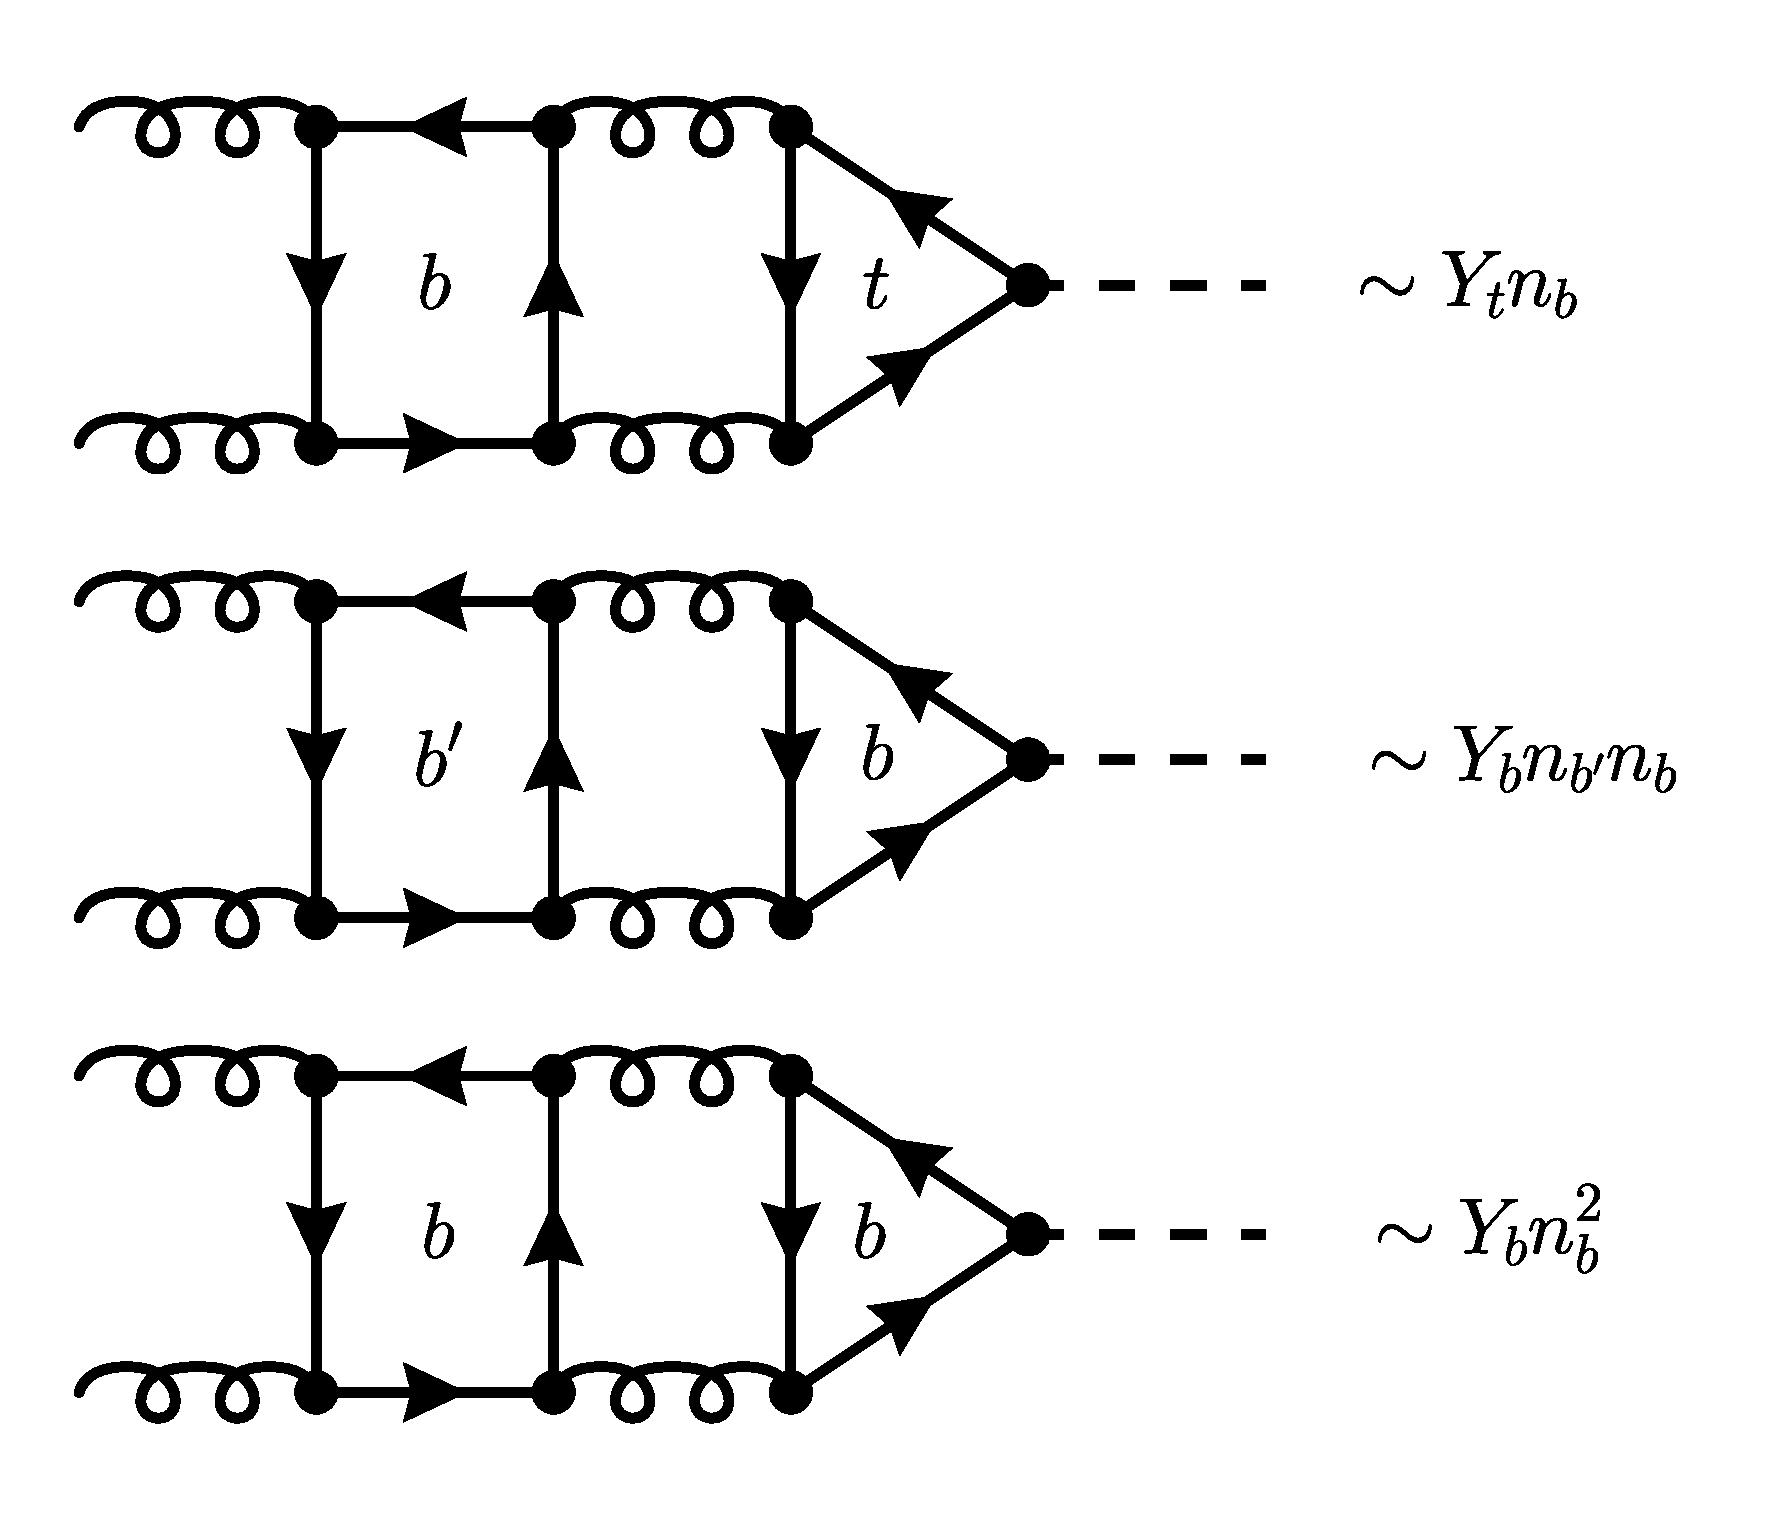
\includegraphics[scale=0.21]{Images/NNLO_Feynman_diagrams/replica.pdf}
\caption{Example Feynman diagrams and their scaling with the Yukawa coupling, $n_b$, and $n_{b^\prime}$.}
\label{fig:5:replica}
\end{figure}
Likewise, after squaring, the contribution $Y_t Y_b n_{b^\prime} n_{b}$ is going to be separately \acs{IR} finite. We have thus shown, that contributions with a massive bottom-quark loop which does \textbf{not} couple to the Higgs does not mix gauge dependent terms or \acs{IR} divergences with the selected contribution from our massification procedure.

\subsection{The Real-Real Corrections}
The real-real corrections only contain a single loop, with either a top or a bottom quark running in the loop. Examples of different Feynman diagrams for various partonic channels are depicted in Fig.~\ref{fig:5:real_real}.
\begin{figure}[h]
  \centering
  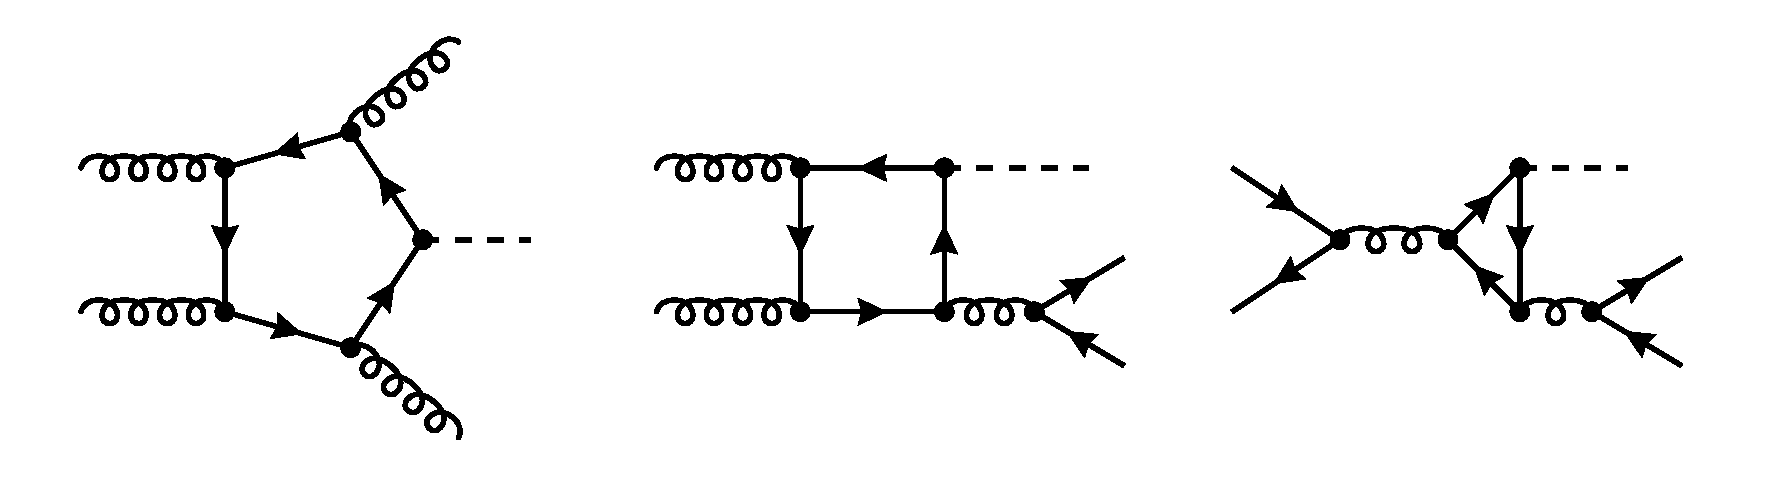
\includegraphics[width=\figurewidth]{Images/NNLO_Feynman_diagrams/RealReal.pdf}
  \caption{Example Feynman diagrams for one-loop real-real corrections in various partonic channels.}
  \label{fig:5:real_real}
\end{figure}

As one-loop amplitudes, they can be computed numerically with publically available libraries like \texttt{Recola}~\cite{Actis:2016mpe}. However, the real-real corrections often represent the bottleneck of the computation of the phase-space integrals, which makes an efficient evaluation of the amplitudes desirable. We therefore instead use the analytic form of the amplitude computed in Ref.~\cite{Budge:2020oyl}. We use the implementation of the amplitudes provided by \texttt{MCFM}~\cite{Campbell:2019dru, Campbell:1999ah, Campbell:2011bn}, which in turn uses \texttt{QCDLoop}~\cite{Ellis:2007qk, Carrazza:2016gav} for the evaluation of one-loop integrals.

We found that with the analytic expressions, the evaluation time of the amplitudes is sped up by a factor of 20 compared to the numerical evaluation in \texttt{Recola}.

\subsection{The Real-Virtual Corrections}
For the real-virtual corrections we, for the first time encounter Feynman diagrams with two different mass scales running in the loop. Fig.~\ref{fig:5:real_virtual2} shows all (up to inversion of the fermion flow inside the triangle loops) Feynman diagrams with two internal quark loops.
\begin{figure}[h]
  \centering
  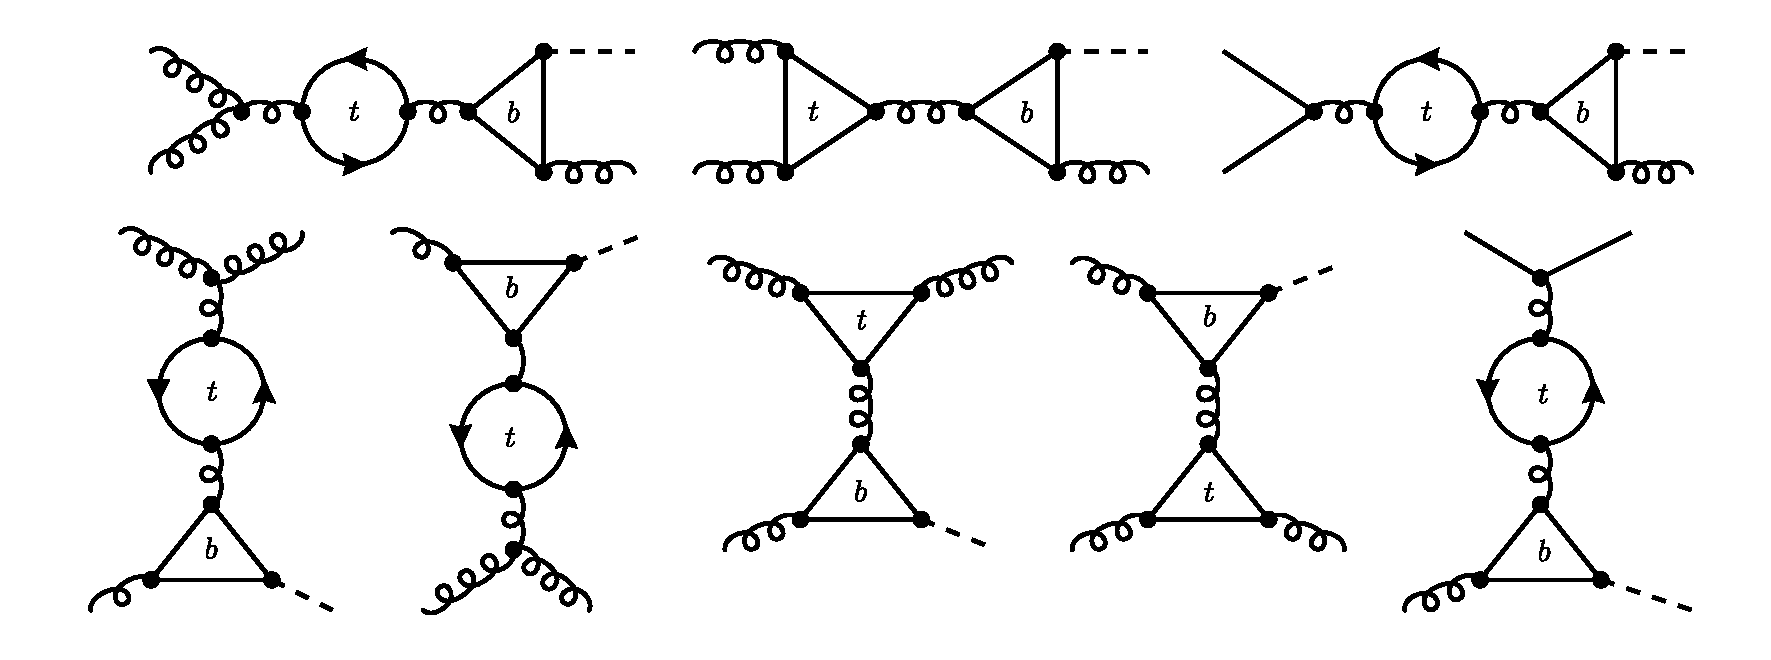
\includegraphics[scale=0.5]{Images/NNLO_Feynman_diagrams/RealVirtual2.pdf}
  \caption{Feynman diagrams for the two-loop real-virtual corrections with two massive quarks. Amplitudes for the $qg \rightarrow Hq$ channel can be obtained via crossing from the $q \bar{q} \rightarrow H g$ amplitudes.Triangle loops with reversed fermion flow are not explicitly shown. The external gluons must be accounted for with all permutations which render a different Feynman diagrams. In the 5\acs{FS}, the bottom-quark is always coupling to the Higgs.}
  \label{fig:5:real_virtual2}
\end{figure}
We observe, that all two-loop integrals actually factorize into two separate one-loop integrals making them quite straight-forward to solve.

The contributions to the scattering amplitude containing only a single massive quark involve genuine two-loop integrals. Fig.~\ref{fig:5:real_virtual1} shows a selection of contributing Feynman diagrams.
\begin{figure}[h]
  \centering
  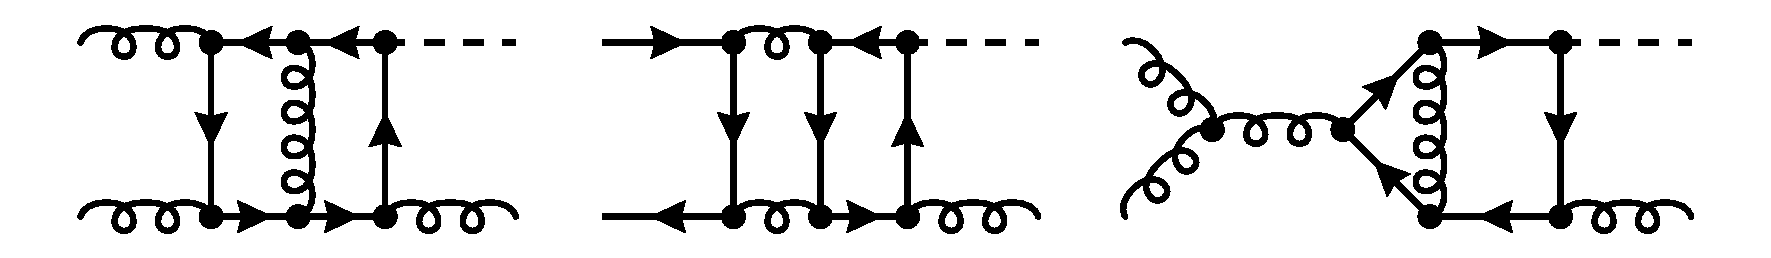
\includegraphics[width=\figurewidth]{Images/NNLO_Feynman_diagrams/RealVirtual1.pdf}
  \caption{Example Feynman diagrams for the two-loop real-virtual corrections with a single massive quark in various partonic channels.}
  \label{fig:5:real_virtual1}
\end{figure}
Two loop integrals, especially non-planar ones, with three mass scales are very challenging to compute analytically, even with state-of-the-art methods, and as of today the analytic computation of these amplitudes are still unknown, however approximations for a nearly massless bottom quark have been calculated relatively recently~\cite{Melnikov:2016qoc, Melnikov:2017pgf}. We therefore decided to instead evaluate the appearing two-loop integrals numerically at fixed phase-space points and interpolate between them during the phase-space integration.

In any case, for both the one-mass and two-masses contribution we first have to reduce the amplitude to form factors. To make possible symmetries more apparent, we cross the radiated parton to the initial state, \ie\ we consider the amplitudes
\begin{equation}
g(p_1) + g_(p_2) + g(p_3) \longrightarrow H(p_4), \qquad \bar{q}(p_1) + q(p_2) + g(p_3) \longrightarrow H(p_4).
\end{equation}

\textbf{Projection to Form Factors}\\
We can factor out the external polarization vectors, spinors and color factors to rewrite the amplitudes in terms of their amputated counterpart
\begin{equation}
\mathcal{M}_{ggg \rightarrow H} = \mathcal{M}_{\mu \nu \rho} \epsilon_1^\mu \epsilon_2^\nu \epsilon_3^\rho f^{c_1 c_2 c_3}, \qquad \mathcal{M}_{\bar{q} q g \rightarrow H} = \bar{v}(p_1) \mathcal{M}_{\rho} u(p_2) \epsilon_3^\rho T^{c_3}_{c_1 c_2}.
\end{equation}
After squaring the amplitude and summing over the color of the external partons, we get the color factors
\begin{equation}
f^{c_1 c_2 c_3} f^{c_1 c_2 c_3} = C_A N_A = 24, \qquad T^{c_3}_{c_1 c_2} T^{c_{3}}_{c_2 c_1} = C_F N_c = 4.
\end{equation}
It is convenient, to choose polarization vectors which are cyclically transverse to the external momenta, \ie\
\begin{equation}
\epsilon_1 = \epsilon (p_1; p_2), \quad \epsilon_2 = \epsilon (p_2; p_3), \quad \epsilon_3 = \epsilon (p_3; p_1),
\end{equation}
where the second argument indicates the gauge vector. We can then propose the form factor decomposition of the amplitudes
\begin{equation}
\begin{split}
\mathcal{M}^{\mu \nu \rho} &= g^{\mu \nu} p_2^\rho F_1 + g^{\mu \rho} p_1^\nu F_2 + g^{\nu \rho} p_3^\mu F_3 + p_3^\mu p_1^\nu p_2^\rho F_4, \\
\bar{v}(p_1) \mathcal{M}^{\rho} u(p_2) &= \bar{v}(p_1)\left[ \slashed{p}_3 p_1^\rho - (p_1 \cdot p_3) \gamma^\rho \right] u(p_2) G_1 + \bar{v}(p_1) \left[ \slashed{p}_3 p_2^\rho - (p_2 \cdot p_3) \gamma^\rho \right] u(p_2) G_2.
\end{split}
\end{equation}
We used the Ward identity, to restrict the tensor coefficients in $\mathcal{M}^\rho$. $\mathcal{M}^{\mu \nu \rho}$ also satisfies Ward identity.

The tensor coefficients span a vector space with respect to the scalar product
\begin{equation}
\braket{a_{\mu_1, \cdots \mu_{n_g}}| b^{\mu_1, \cdots \mu_{n_g}}} \equiv \sum_{\text{pol.}} a^*_{\mu_1 \ldots \mu_{n_g}} \left[\prod_i^{n_g} \epsilon_i^{*\mu_i} \epsilon_i^{\nu_i}  \right]  b_{\nu_1 \ldots \nu_{n_g}}
\label{eq:5:scala_product}
\end{equation}
where $n_g$ is the number of external gluons, \ie $n_g = 3$ for $ggg \rightarrow H$ and $n_g = 1$ for $\bar{q} q g \rightarrow H$ and the summation is performed over the polarizations of all external particles. The tensor coefficients hence form a---not necessary orthonormal---basis.

Any vector can be written as a linear sum over basis vectors
\begin{equation}
\ket{v} = \sum_i v_i \ket{e_i}.
\end{equation}
Then the projector to the $j$-th basis vector can be found via
\begin{equation}
\bra{e_j}P \equiv P_j = \sum_k G^{-1}_{jk} \ket{e_k},
\end{equation}
where $G$ is the Gram-matrix
\begin{equation}
G_{ij} = \braket{e_i | e_j}.
\end{equation}

With this little interlude from linear algebra it is then easy to verify that the projectors for the $F_1,\ldots , F_4$ form factors are given by
\begin{equation}
\begin{split}
P_1^{\mu \nu \rho} &= \frac{1}{d - 3} \left( g^{\mu \nu} p_2^\rho \frac{t}{su} - p_3^\mu p_1^\nu p_2^\rho \frac{1}{su} \right), \\
P_2^{\mu \nu \rho} &= \frac{1}{d - 3} \left( g^{\mu \rho} p_1^\nu \frac{u}{s t} - p_3^\mu p_1^\nu p_2^\rho \frac{1}{st} \right), \\
P_3^{\mu \nu \rho} &= \frac{1}{d - 3} \left( g^{\nu \rho} p_3^\mu \frac{s}{t u} - p_3^\mu p_1^\nu p_2^\rho \frac{1}{t u} \right), \\
P_4^{\mu \nu \rho} &= \frac{1}{d - 3} \left( - g^{\mu \nu} p_2^\rho \frac{1}{s u} - g^{\mu \rho} p_1^\nu \frac{1}{s t} - g^{\nu \rho} p_3^\mu \frac{1}{t u} + p_3^\mu p_1^\nu p_2^\rho \frac{d}{s t u} \right).
\end{split}
\end{equation}
To be even more explicit: the form factors are given by
\begin{equation}
\begin{split}
&F_i = \braket{e_i| P_{\mu \nu \rho} | \mathcal{M}^{\mu \nu \rho}} = P_i^{\mu_1 \nu_1 \rho_1} \left(-g_{\mu_1 \mu_2} + \frac{p_{1\, \mu_1} p_{2\, \mu_2} + p_{2\, \mu_1} p_{1\, \mu_2}}{p_1 \cdot p_2} \right) \\
& \qquad \times \left(-g_{\nu_1 \nu_2} + \frac{p_{2\, \nu_1} p_{3\, \nu_2} + p_{3\, \nu_1} p_{2\, \nu_2}}{p_2 \cdot p_3} \right) \left(-g_{\rho_1 \rho_2} + \frac{p_{3\, \rho_1} p_{1\, \rho_2} + p_{1\, \rho_1} p_{3\, \rho_2}}{p_3 \cdot p_1} \right) \mathcal{M}^{\mu_2 \nu_2 \rho_2}.
\end{split}
\end{equation}
Here we used the standard identity
\begin{equation}
\sum_{\lambda} \epsilon^{*}_\mu (p, n, \lambda) \epsilon_\nu(p, n, \lambda) = -g_{\mu \nu} + \frac{p_\mu n_\nu + p_\nu n_\mu}{p \cdot n}
\end{equation}
to rewrite the sum over the polarization vectors.

Similarly, using
\begin{equation}
\sum_{\lambda} u(p, \lambda) \bar{u}(p, \lambda) = \slashed{p}, \quad \text{and} \quad \sum_\lambda v(p, \lambda) \bar{v}(p, \lambda) = \slashed{p},
\label{eq:5:spinor_polarization_sum}
\end{equation}
we find the projectors of $G_1$ and $G_2$\footnote{Note that the projectors are defined as the entire left-hand side.}
\begin{equation}
\begin{split}
\bar{v}(p_1) P_1^\mu u(p_2) &= \frac{1}{2 s t (d - 3)} \bar{v}(p_1) \left[ \frac{d - 2}{t} \left(\slashed{p}_3 p_1^\mu - \frac{t}{2} \gamma^\mu \right) - \frac{d - 4}{u} \left(\slashed{p}_3 p_2^\mu - \frac{u}{2} \gamma^\mu \right) \right]u(p_2), \\
\bar{v}(p_1) P_2^\mu u(p_2) &= \frac{1}{2 s u (d - 3)} \bar{v}(p_1) \left[ \frac{d - 2}{u} \left(\slashed{p}_3 p_2^\mu - \frac{u}{2} \gamma^\mu \right) - \frac{d - 4}{t} \left(\slashed{p}_3 p_1^\mu - \frac{t}{2} \gamma^\mu \right) \right] u(p_2). \\
\end{split}
\end{equation}
These allow the extraction of the form factors via
\begin{equation}
\begin{split}
G_i = \braket{e_i| P_\mu |\mathcal{M}^\mu} =  \left(-g_{\mu_1 \mu_2} + \frac{p_{3\, \mu_1} p_{1\, \mu_2} + p_{1\, \mu_1} p_{3\, \mu_2}}{p_3 \cdot p_1} \right) \text{tr} \big \lbrace P_i^{\mu_1} \mathcal{M}^{\mu_2} \big \rbrace,
\end{split}
\end{equation}
where we have used Eq.~\eqref{eq:5:spinor_polarization_sum} once again, to rewrite the polarization sum in terms of a Dirac-trace.

\textbf{Helicity Amplitudes} \\
Since the form factors dependent on the choice of our tensor basis, we would rather express our end result in terms of helicity amplitudes
\begin{equation}
\begin{split}
\mathcal{M}^{\lambda_1 \lambda_2 \lambda_3}_{ggg \rightarrow H} &= \mathcal{M}_{\mu \nu \rho} \epsilon^\mu(p1, p_2, \lambda_1) \epsilon_2^\nu(p_2, p_3, \lambda_2) \epsilon_3^\rho(p_3, p_1, \lambda_3), \\
\mathcal{M}^{\lambda_1 \lambda_2 \lambda_3}_{\bar{q}q g \rightarrow H} &= \bar{v}(p_1, \lambda_1/2) \mathcal{M}_{\rho} u(p_2, \lambda_2/2)  \epsilon_3^\rho(p_3, p_1, \lambda_3).
\end{split}
\end{equation}
To find the relation between the form factors and the helicity amplitudes, we consider all independent helicity configurations and use the \textit{spinor-helicity formalism} (see Ref.~\cite{Dixon:1996wi} for a pedagogical introduction to the topic) to rewrite them in terms of spinor products
\begin{equation}
\braket{ij} \equiv \bar{u}(p_i, -1/2) u(p_j, 1/2), \qquad [ij] \equiv \bar{u}(p_i, 1/2) u(p_j, -1/2).
\end{equation}
The results for the $ggg \rightarrow H$ amplitudes read
\begin{equation}
\begin{split}
\mathcal{M}_{ggg\rightarrow H}^{+++} &= \frac{1}{\sqrt{2}} \frac{s u}{\braket{12} \braket{23} \braket{31}} \left( F_1 + \frac{t}{u} F_2 + \frac{t}{s} F_3 + \frac{t}{2} F_4 \right), \\
\mathcal{M}_{ggg\rightarrow H}^{++-} &= \frac{1}{\sqrt{2}} \frac{[12]^3}{[13][23]} \frac{u}{s} \left(F_1 + \frac{t}{2} F_4 \right), \\
\mathcal{M}_{ggg\rightarrow H}^{+-+} &= \frac{1}{\sqrt{2}} \frac{[13]^3}{[12][23]} \frac{s}{t} \left(F_2 + \frac{u}{2} F_4 \right), \\
\mathcal{M}_{ggg\rightarrow H}^{-++} &= \frac{1}{\sqrt{2}} \frac{[23]^3}{[12][13]} \frac{t}{u} \left(F_3 + \frac{s}{2} F_4 \right).
\end{split}
\end{equation}
The other four helicity amplitudes can be determined via charge conjugation
\begin{equation}
\mathcal{M}^{\lambda_1, \lambda_2, \lambda_3} = \mathcal{M}^{-\lambda_1, - \lambda_2, -\lambda_3} \big \vert_{\braket{ij} \leftrightarrow [ji]}.
\label{eq:5:parity}
\end{equation}
Similarly, for the $\bar{q}q g \rightarrow H$ process we find the helicity amplitudes
\begin{equation}
\begin{split}
\mathcal{M}^{-++}_{\bar{q}q g \rightarrow H} &= - \frac{1}{\sqrt{2}} \frac{[13]^2}{[12]} s F_1, \\
\mathcal{M}^{+-+}_{\bar{q}q g \rightarrow H} &= \frac{1}{\sqrt{2}} \frac{[23]^2}{[12]} s F_2.
\end{split}
\end{equation}
The $+--$ and $-+-$ amplitudes can be determined with Eq.~\eqref{eq:5:parity} and all other helicity configurations render vanishing amplitudes due to the conservation of angular momentum.

The form factors, amplitudes and helicity amplitudes admit a perturbative expansion in $\alphas$. We define
\begin{equation}
\mathcal{M}^{\lambda_1\lambda_2 \lambda_3}_{ijk \rightarrow H} = \frac{4 \pi}{v}  \left(\alphas\right)^{3/2} \sum_{i = 0} \left(\frac{\alphas}{4 \pi} \right)^i \mathcal{M}^{(i),\lambda_1 \lambda_2 \lambda_3}.
\end{equation}
\textbf{Mapping to Topologies and the Reduction to Master Integrals} \\
We generate all diagrams with \texttt{DiaGen/IdSolver}, our in-house software tool for the generation of Feynman diagrams. As output, we obtain \texttt{FORM}~\cite{Vermaseren:2000nd, Ruijl:2017dtg} code we can further manipulate. We apply the color algebra and project to the form factors as described above. \texttt{DiaGen/IdSolver} is also capable to find \textit{prototypes}, \ie\ it automatically identifies a minimal set of integral families and assigns appearing integrals accordingly.

In principle, \texttt{DiaGen/IdSolver} is also able to find relations between appearing Feynman integrals, so called \textit{integration-by-parts identities} (\acs{IBP}), by means of the \textit{Laporta algorithm}~\cite{Laporta:2000dsw}. However, due to the immense complexity of the problem at hand, intermediate expressions are prone to become very large. This makes solving the appearing linear system of equation by traditional methods like Gaussian elimination highly inefficient. The appearance of large intermediate expressions can be circumvented by using \textit{finite field} methods. In a nutshell, one inserts fractional samples for the appearing kinematic invariants and then performs the Laporta algorithm with reduced kinematics, making it much simpler to solve. The final \acs{IBP} identities relate the master integrals by rational functions, one can then reconstruct the functional dependence on the kinematic variables through repeated sampling, like when performing a fit. The rational values are mapped to finite fields---explaining the name of the method---which allows computations without loss of precision. We use this workflow implemented in the publically available tool chain \texttt{Kira$\,\oplus\,$Firefly}~\cite{Maierhofer:2017gsa, Maierhofer:2018gpa, Klappert:2020nbg}.

After application of the \acs{IBP} identities we end up with three integral families for amplitudes with a single internal massive quark. We adapt the definition provided in Ref.~\cite{Melnikov:2016qoc}. The propagators of the each family are printed in Tab.~\ref{tab:5:integral_families}.
\begin{table}[h]
\centering
\begin{tabular}{clll}
\# & Planar 1 (PL1) & Planar 2 (PL2) & Non-planar (NPL) \\
\hline
1 & $k_1^2$ & $k_1^2 - m^2$ & $k_1^2 - m^2$ \\
2 & $(k_1 - p_1)^2$ & $(k_1 - p_1)^2 - m^2$ & $(k + p_1)^2 - m^2$ \\
3 & $(k_1 - p_1 - p_2)^2$ & $(k_1 - p_1 - p_2)^2 - m^2$ & $(k_1 - p_2 - p_3)^2 - m^2$ \\
4 & $(k_1 - p_1 - p_2 - p_3)^2$ & $(k_1 - p_1 - p_2 - p_3)^2 - m^2$ & $k_2^2 - m^2$ \\
5 & $k_2^2 - m^2$ & $k_2^2 - m^2$ & $(k_2 + p_1)^2 - m^2$ \\
6 & $(k_2 - p_1)^2 - m^2$ & $(k_2 - p_1)^2 - m^2$ & $(k_2 - p_3)^2 - m^2$ \\
7 & $(k_2 - p_1 - p_2)^2 - m^2$ & $(k_2 - p_1 - p_2)^2 - m^2$ & $(k_1 - k_2)^2$ \\
8 & $(k_2 - p_1 - p_2 - p_3)^2 - m^2$ & $(k_2 - p_1 - p_2 - p_3)^2 - m^2$ & $(k_1 - k_2 - p_2)^2$ \\
9 & $(k_1 - k_2)^2 - m^2$ & $(k_1 - k_2)^2$ & $(k_1 - k_2 - p_2 - p_3)^2$
\end{tabular}
\caption{Integral families for all contributions with only one internal massive quark as defined in Ref.~\cite{Melnikov:2016qoc}. $m$ is the mass of the internal top- or bottom-quark.} \label{tab:5:integral_families}
\end{table}
Notice, that the Feynman diagrams can never have more than seven internal lines, meaning that integrals appearing in physical amplitudes are missing at least two of the propagators. The physical subsector of the integral families are depicted graphically in Figs.~\ref{fig:5:PL1}, \ref{fig:5:PL2}, and \ref{fig:5:NPL}.
\begin{figure}[h]
\centering
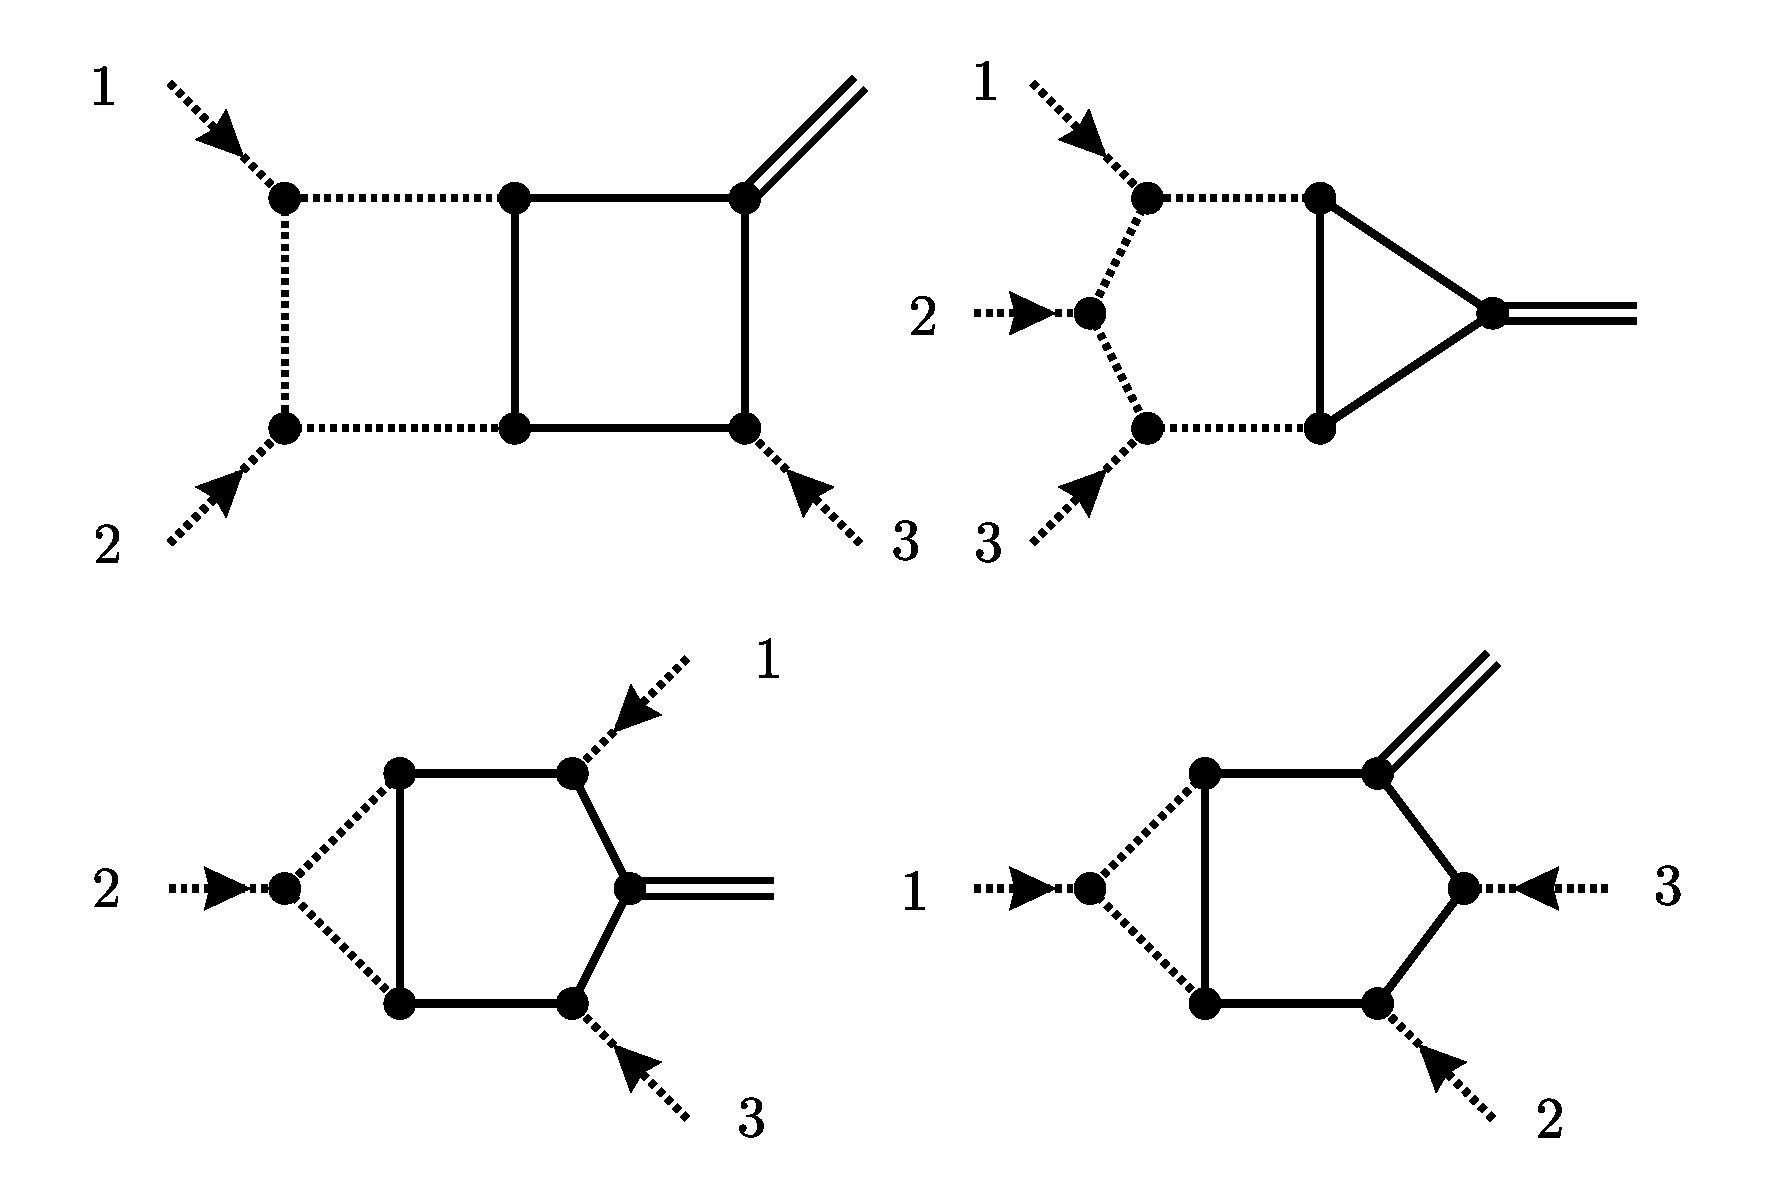
\includegraphics[scale=0.3]{Images/NNLO_Feynman_diagrams/PL1.pdf}
\caption{Graphical representation of the physical sectors embedded in the first integral family (PL1). Dotted lines represent massless propagators, while solid lines have the quark mass in the propagator.} \label{fig:5:PL1}
\end{figure}
\begin{figure}[h]
\centering
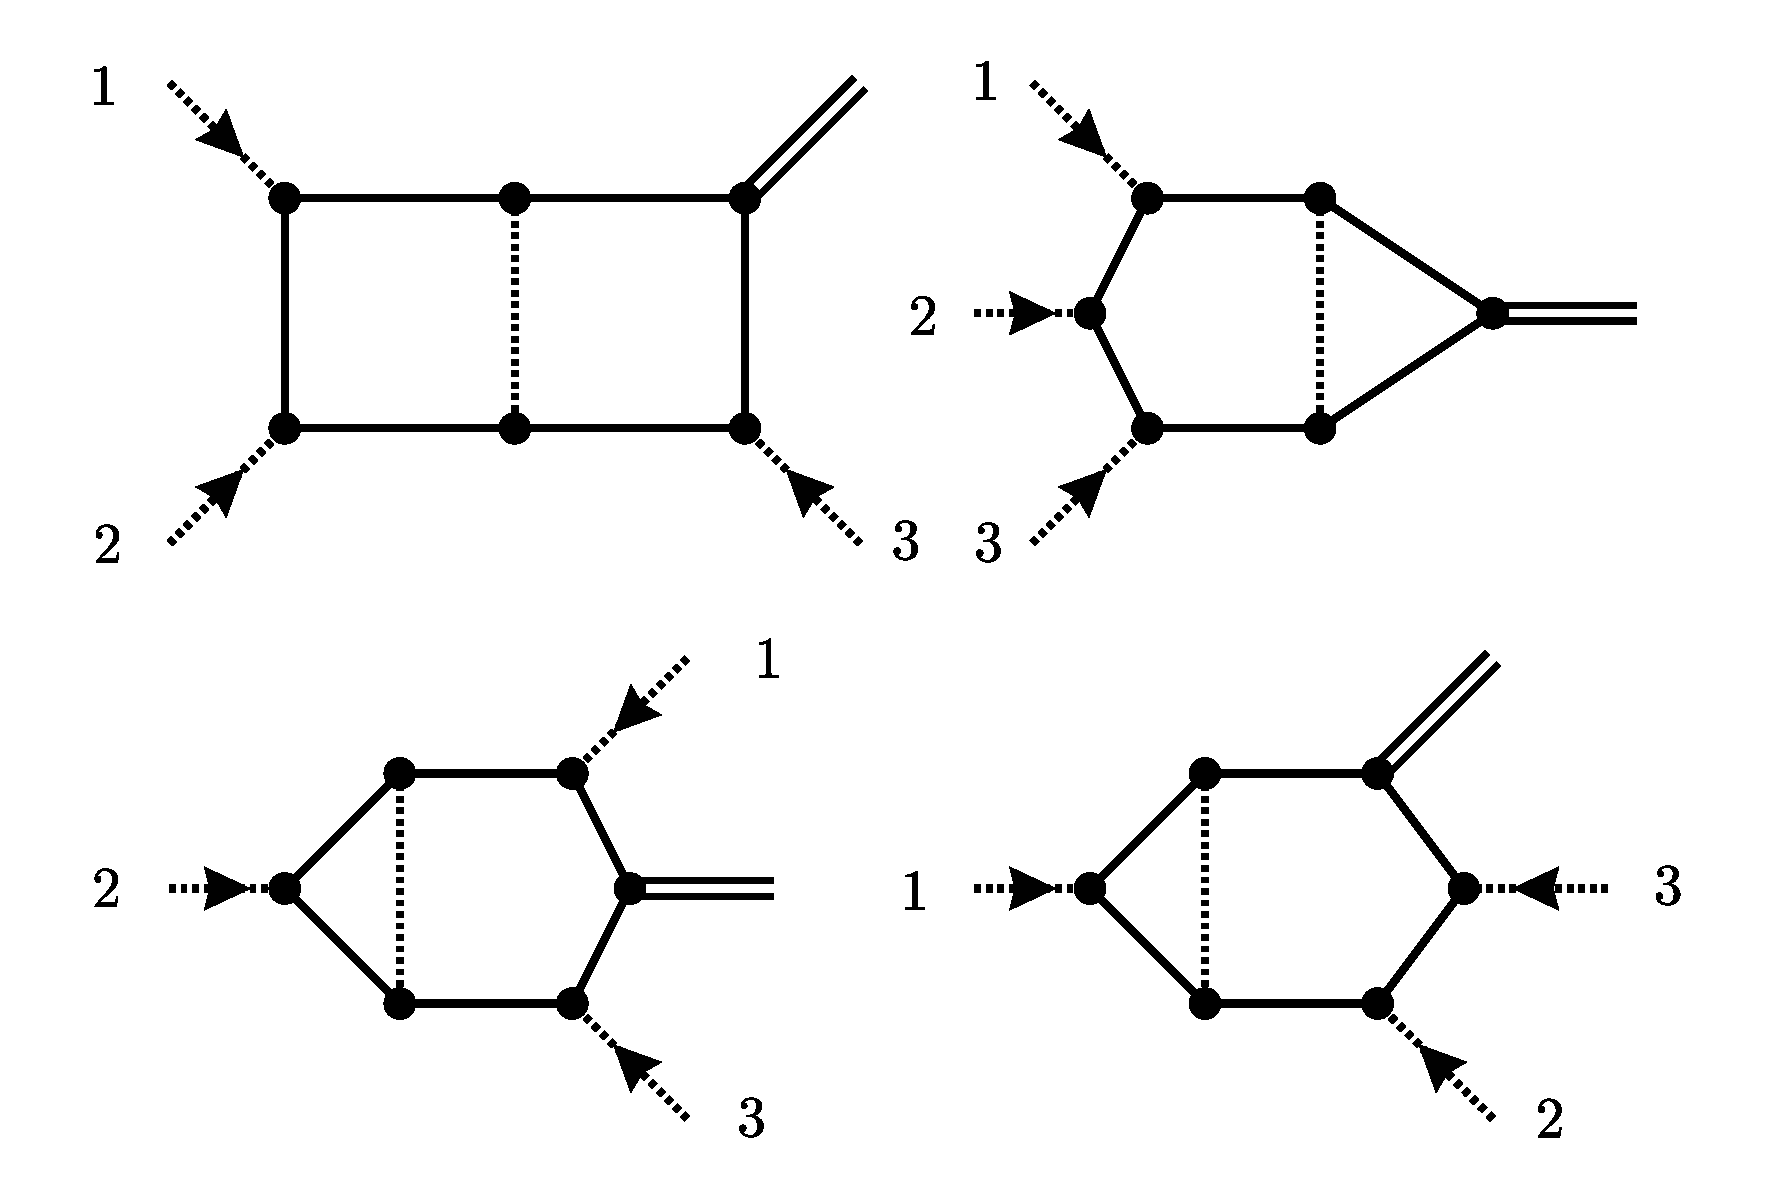
\includegraphics[scale=0.3]{Images/NNLO_Feynman_diagrams/PL2.pdf}
\caption{Same as Fig.~\ref{fig:5:PL1} but for the second integral family (PL2).} \label{fig:5:PL2}
\end{figure}
\begin{figure}[h]
\centering
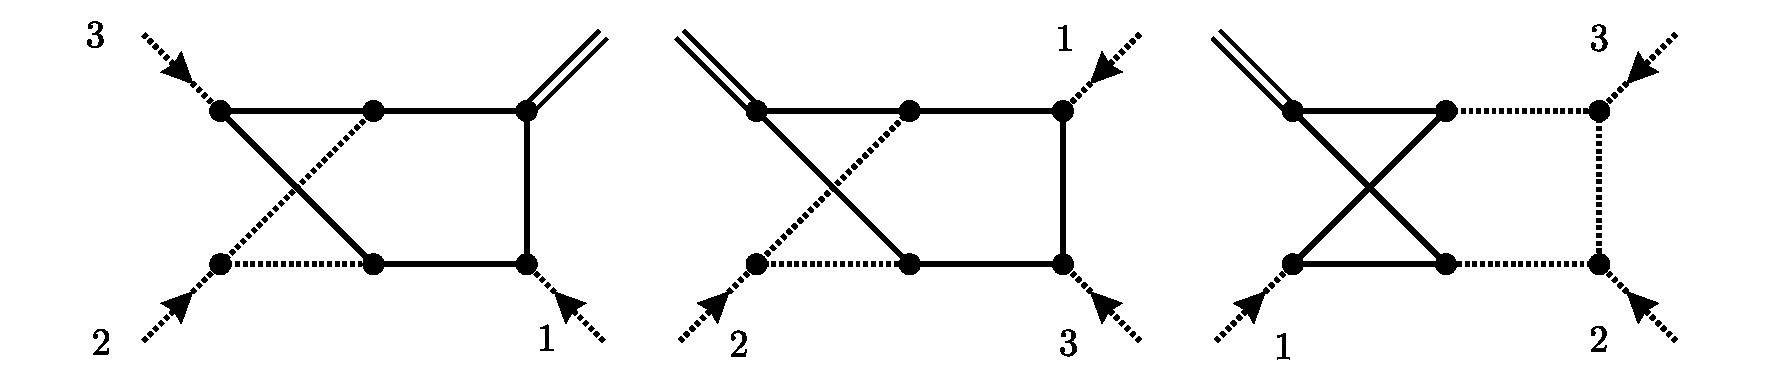
\includegraphics[scale=0.4]{Images/NNLO_Feynman_diagrams/NPL.pdf}
\caption{Same as Fig.~\ref{fig:5:PL1} but for the third non-planar integral family (NPL).} \label{fig:5:NPL}
\end{figure}
For the contributions containing two massive internal quarks, we do not provide the integral families since the two-loop integrals factorize to one-loop integrals.

\textbf{\acs{UV}-Renormalization, \acs{IR}-Subtraction and LSZ-Reduction} \\
So far our analysis was concerned with bare amplitudes regulated in dimensional regularization. The \acs{UV}-poles are eliminated through renormalization of the coupling constant and the quark masses. Following the description in section~\ref{sec:2:cross_sections} we replace the bare coupling constant and masses by their renormalized counterparts and subsequently expand in $\alphas$. The $\alphas^{5/2}$ term is singled out to get the \acs{NNLO} correction to the amplitude. We employ the \MS\ scheme for the $\alphas$, and---for now---the OS scheme for all the quark masses.

To obtain physical amplitudes, we employ the LSZ reduction formula. This means for each external particle, multiplying by the square root of the corresponding LSZ-constant. In dimensional regularization, the LSZ constants only get contributions from heavy fields, since all other contributions render scaleless integrals. This means that the gluon LSZ constants are already non-trivial at one-loop, whereas the quark LSZ constants only gets non-trivial corrections at two-loop, which makes them irrelevant for the calculation at hand. Since bottom-quarks are treated as massless whenever they are not coupling to the Higgs, they do not contribute to the LSZ constants, \ie\ only the top-quark mass enters the LSZ constants.

The remaining poles are of \acs{IR} origin. They would cancel against poles arising during phase-space integration, so we can subtract them already on the amplitude level. We employ the \MS\ scheme and subtract only the divergences predicted by the $\mathbf{Z}$ operator (see for example Ref.~\cite{Czakon:2014oma}).

\textbf{Results for the Contributions with Two Heavy Quarks} \\
Once we performed all the above steps, we separate the contributions which contain two heavy quark loops from the rest of the amplitude. The $\mathbf{Z}$ operator, \ie\ the \acs{IR}-poles, do not receive contributions from heavy internal lines and is therefore irrelevant for this contribution. The LSZ constants of the gluons on the other hand, do contribute. In the coupling renormalization constants, we single out the contributions from the top quark, \ie\ we set the number of fermions to
\begin{equation}
n_f = n_l + n_h
\end{equation}
Here $n_l$ is the number of light quarks, and $n_h$ is the number of heavy quarks. In the 5\acs{FS} we have $n_l = 5$ and $n_h = 1$. The renormalization constant in the \MS\ scheme then reads
\begin{equation}
Z_g = 1 - \frac{\alphas}{4 \pi}  2 \beta_0 \frac{1}{\epsilon} + \BigO{\alphas^2} = 1 + \frac{\alphas}{4 \pi} \frac{1}{\epsilon} \left(- \frac{11}{6} C_A + \frac{2}{3} (n_l + n_h) T_F \right) + \BigO{\alphas^2}.
\end{equation}
To single out the contributions from the top-quark we only take terms proportional to $n_h$ and set $n_h$ to one afterwards. We can then apply the decoupling relations of Eq.~\eqref{eq:4:decoupling} to replace the coupling constant by its decoupled counterpart in the lower order amplitudes\footnote{In the renormalization constants we can simply set $\alphas^{(n_l + n_h)} = \alphas^{(n_l)}$ at this order in perturbation theory.}. We can absorb these terms into the renormalization of the coupling constant, such that we end up with the effective renormalization constant
\begin{equation}
Z_g^{(n_l)} \big \vert_{\propto n_h} = \frac{\alphas}{4 \pi} \frac{2}{3} T_F \left(\frac{1}{\epsilon} - \ln\!\left(\frac{m_t^2}{\mu^2}\right) \right) + \BigO{\alphas^2}.
\end{equation}
This is nothing else than the top-quark contribution to the \acs{OS} coupling renormalization constant. The decoupling constants were specifically introduced to cure the \MS\ scheme from the appearance of non-decoupling effects. In the \acs{OS} scheme this issue does not arise because of the Appelquist-Carrazone theorem (see section~\ref{subsec:4:matching_of_wilson_coefficients}). It therefore comes to no ones surprise that the effective renormalization constant matches the OS one.

At one-loop, the top-quark contribution to the renormalization constant is of abelian nature. In \acs{QED}, the Ward identity implies the all order relation $Z_e = Z_3^{-1/2}$. We can therefore conclude, or verify explicitly that the one-loop renormalization constant is also related to the gluon LSZ constant
\begin{equation}
2 Z_g^{(n_l)} \big \vert_{\propto n_h} = - Z_3 + \BigO{\alphas^2}.
\end{equation}
This has the profound effect, that if the external number of gluons is identical to the power of the coupling constant (at lower order), then the contributions exactly cancel. This is for example the case in the $ggg \rightarrow H$ amplitude.

The result for the helicity amplitude of the $ggg \rightarrow H$ amplitude read
\begin{equation}
\begin{split}
&\mathcal{M}^{(1),+++}_{ggg \rightarrow H} \bigg \vert_{2\ \text{masses}} = \frac{1}{\sqrt{2}} \frac{1}{\braket{12}\braket{23} \braket{31}} \bigg \lbrace -  \frac{4 m_t^2 s t u}{(s + t)} \tilde{C}_0\!(u, m_t^2) \bigg [ \tilde{B}\!(m_H^2, m_b^2)  \\
& \hspace{2cm} + \frac{s + t}{u} + 2 \frac{m_b^2}{u} \left( 4 m_b^2 - s - t \right) \tilde{C}_1\!(u, m_H^2, m_b^2) - \frac{4 m_b^2}{s + t} \tilde{B}(u, m_l^2)  \bigg ] \\
& \hspace{5cm} + (s \rightarrow t, t \rightarrow u, u \rightarrow s) + (s \rightarrow u, u \rightarrow t, t \rightarrow s)\bigg \rbrace
\label{eq:5:ggg_ppp}
\end{split}
\end{equation}
%
%
\begin{equation}
\begin{split}
&\mathcal{M}^{(1),-++}_{ggg \rightarrow H} \bigg \vert_{2\, \text{masses}} = -\frac{1}{\sqrt{2}} \frac{[23]^3}{[12][13]} \frac{4 m_t^2 s t }{u(s + t)} \tilde{C}_0\!(u, m_t^2) \bigg [ \tilde{B}\!(m_H^2, m_b^2) \\
& \hspace{2cm} + \frac{s + t}{u} + 2 \frac{m_b^2}{u} \left(4 m_b^2 - s - t\right) \tilde{C}_1\!(u, m_H^2, m_b^2) - \frac{4 m_b^2}{(s + t)} \tilde{B}\!(u, m_b^2) \bigg ]
\label{eq:5:ggg_mpp}
\end{split}
\end{equation}
Where we defined the auxiliary functions\footnote{The functions are closely related to the finite part of the bubble integrals, and the triangle integrals with on-shell, and one off-shell leg. The functions are modified slightly to simplify the expressions, however we keep the standard notation, where $B$ functions indicate bubbles and $C$ functions triangle integrals. The tilde is added to make the distinction from the original integrals more apparent.}
\begin{equation}
\begin{split}
\tilde{B}\!(s, m^2) &\equiv \beta(s, m^2) \log\!\left(- \frac{1 - \beta(s, m^2)}{1 + \beta(s, m^2)} + i 0^+ \right), \\
\tilde{C}_0\!(s, m^2) &\equiv \frac{1}{2 s} \log^2\!\left(- \frac{1 - \beta(s, m^2)}{1 + \beta(s, m^2)} + i 0^+ \right) + \frac{2}{s} \left(\tilde{B}\!(s, m^2) + 2 \right), \\
\tilde{C}_1\!(s_1, s_2, m^2) &\equiv \frac{1}{2} \frac{1}{s_1 - s_2} \left[ \log^2\!\left(-\frac{1 - \beta(s_1, m^2)}{1 + \beta(s_2, m^2)} + i 0^+ \right) - \log^2\!\left(- \frac{1 - \beta(s_2, m^2)}{1 + \beta(s_2, m^2)} + i0^+\right) \right], \\
\text{with} \quad \beta(s, m^2) &\equiv \sqrt{1 - \frac{4 m^2}{s}}.
\label{eq:5:function_definitions}
\end{split}
\end{equation}
All other helicity amplitudes are either related via charge conjugation \eqref{eq:5:parity}, or by relabeling of the external momenta
\begin{equation}
\mathcal{M}_{ggg \rightarrow H}^{+-+} = \mathcal{M}_{ggg \rightarrow H}^{-++} \bigg \vert_{p_1 \leftrightarrow p_2}, \qquad \mathcal{M}_{ggg \rightarrow H}^{++-} = \mathcal{M}_{ggg \rightarrow H}^{-++} \bigg \vert_{p_1 \leftrightarrow p_3}.
\end{equation}
Note that the Mandelstam variables are defined in terms of incoming gluon momenta, \ie\
\begin{equation}
s = (p_1 + p_2)^2, \quad t = (p_1 + p_3)^2, \quad u = (p_2 + p_3)^2.
\end{equation}
For the quark channel the result reads
\begin{equation}
\begin{split}
&\mathcal{M}_{\bar{q}q g \rightarrow H}^{(1),-++} \bigg \vert_{2\, \text{masses}} =  \frac{1}{\sqrt{2}} \frac{[13]^2}{[12]}  \frac{4 }{9 (t + u)} \left(5 s + 12 m_t^2 + (3 s + 6 m_t^2) \tilde{B}\!(s, m_t^2) \right)\bigg [\tilde{B}\!(m_H^2, m_b^2) \\
& \hspace{2cm}  + \frac{t + u}{s} + 2 \frac{m_b^2}{s} \left(4m_b^2 - t - u  \right) \tilde{C}_1\!(s, m_H^2, m_b^2) - \frac{4 m_b^2}{t + u}\tilde{B}\!(s, m_b^2) \bigg ].
\label{eq:5:qqg_mpp}
\end{split}
\end{equation}
Once again all other amplitudes can be obtained through a relabeling of the external momenta and charge conjugation. We see that the functional dependence on the Mandelstams is identical in all amplitudes in Eqs.~\eqref{eq:5:ggg_ppp}, \eqref{eq:5:ggg_mpp}, and \eqref{eq:5:qqg_mpp}. This is because the expression is related to the off-shell gluon-Higgs form factor, appearing in all Feynman diagrams of this contribution (see Fig.~\ref{fig:5:real_virtual2}).

\textbf{Contributions With One Heavy Quark} \\
For completeness, we also reproduce the \acs{LO} helicity amplitudes computed in Ref.~\cite{Baur:1989cm}.
\begin{equation}
\begin{split}
& \mathcal{M}_{ggg \rightarrow H}^{(0), +++} = \frac{1}{\sqrt{2}} \frac{16 m^2 stu}{\braket{12}\braket{23}\braket{31}} \bigg \lbrace - 8 \left[ \frac{1}{u t} + \frac{1}{t t_1} + \frac{1}{u u_1} \right] - \frac{8}{s} \left[ \frac{2 s + t}{u_1^2} B_1(u) + \frac{2 s + u}{t_1^2} B_1(t) \right] \\
& \qquad - \frac{2 (s - 4 m^2)}{stu} \left[ s_1 C_1(s) + (u - s) C_1(t) + (t - s) C_1(u) \right] - 16 m^2 \left[ \frac{1}{t t_1} C_1(t) + \frac{1}{u u_1} C_1(u) \right] \\
& \qquad + \frac{8 m^2}{s} D(u, t) + \frac{s - 4 m^2}{s t u} \left[ s t D(s, t) + u s D(u, s) - u t D(u, t) \right] - \frac{4}{s^2} E(u, t) \bigg \rbrace
\end{split}
\end{equation}
%
%
\begin{equation}
\begin{split}
& \mathcal{M}_{ggg \rightarrow H}^{(0), -++} = \frac{1}{\sqrt{2}} \frac{[23]^3}{[12][13]} \frac{16 m^2 s t}{u} \bigg \lbrace \frac{8 m_H^2}{s t u} + \frac{2 (m_H^2 - 4 m^2)}{stu} \left[ s_1 C_1(s) + u_1 C_1(u) + t_1 C_1(t) \right] \\
&\qquad - \frac{m_H^2 - 4 m^2}{stu} \left[ s t D(s, t) + u s D(u, s) + u t D(u, t) \right] \bigg \rbrace
\end{split}
\end{equation}
%
%
\begin{equation}
\mathcal{M}_{\bar{q} q \rightarrow H}^{(0), -++} = \frac{1}{\sqrt{2}} \frac{[13]^2}{[12]} \frac{m^2}{s_1} \left[ 2 + 2 \frac{s}{s_1} B_1(s) + \left(4 m^2 - u - t \right) C_1(s) \right]
\end{equation}
Here $m$ is the internal quark mass and we defined
\begin{equation}
s_1 = s - m_H^2, \quad t_1 = t - m_H^2, \quad u_1 = u - m_H^2.
\end{equation}
The appearing functions are directly linked to standard Feynman integrals which we provide in Appendix~\ref{app:2}.
\todo{Check numerically}

Although there is one less scale in the contributions with only one quark mass, the two-loop amplitudes are a lot more complex because the integrals do no longer factorize. Instead of attempting to solve the remaining integrals analytically, we followed a numerical approach, where the amplitudes are evaluated at fixed phase-space points. These points can then be used as grid points for interpolations during the phase-space integration. For the numerical evaluation of the master integrals we follow the strategy outlined in Ref.~\cite{Czakon:2021yub}, which itself is based on methods presented in Ref.~\cite{Czakon:2015exa}. The general idea is to derive a system of differential equation for each integral family, find suitable boundary conditions analytically, and then solve the differential equations numerically.

The amplitude is a function of four variables, \eg\ $s, t, u$ and the quark mass $m$. The Higgs mass is not a free parameter since it can be expressed as a sum over the Mandelstams. We can however simply factor our one scale, say the collision scale $s$ to make everything dimensionless, and we are left with only three. We choose to parametrize the amplitude in terms of the dimensionless variables
\begin{equation}
z \equiv - \frac{t + u}{s}, \quad \lambda \equiv \frac{t}{t + u}, \quad x \equiv \frac{m^2}{s} = \frac{m^2}{m_H^2} (1 - z).
\end{equation}
These variables are advantageous because they parametrize soft and collinear limits. Indeed, soft limits are described with $z \rightarrow 0$, whereas the collinear limits are captured by $\lambda \rightarrow 0$ for the $t$-collinear and $\lambda \rightarrow 1$ for $u$-collinear. Furthermore, $z$ and $\lambda$ are bounded by
\begin{equation}
0 \le z \le 1, \quad 0 \le \lambda \le 1, \quad \text{and} \quad 0 \le x
\end{equation}
for physical production kinematics.

To apply the method of differential equations, we need to apply derivatives with respect to our variables, but the master integrals are functions of the external momenta. We can apply the chain rule to relate the derivatives
\begin{equation}
\begin{split}
\left(z \frac{\partial }{\partial z} \right) &= \left(t \frac{\partial }{ \partial t} \right) + \left( u \frac{\partial}{ \partial u} \right) + \frac{t + u}{s + t + u} \left(x \frac{\partial}{ \partial x} \right) \\
&= \left(p_3^\mu \frac{\partial}{\partial p_3^\mu} \right) - \frac{z}{1 - z} \left(x \frac{\partial }{\partial x} \right),
\end{split}
\end{equation}


\subsection{The Virtual-Virtual Corrections}
\section{\texorpdfstring{$\MS$}{MS}-scheme}
\section{The 4-Flavour Scheme}\label{sec:5:4FS}
\section{Performing the Phase-Space Integration}


